\chapter{Theorie}

\section{SetlX}

\section{MNIST}

\section{Perceptrons}
Ein Perceptron ist ein mathematisches Modell zur Abbildung eines künstliches Neurons in einem Netzwerk. Es wird für die Entscheidungsfindung herangezogen, indem verschiedene Aussagen abgewägt werden. Hierbei nimmt das Perceptron eine Menge von Eingaben $x_n$ mit $n \in \{1, \cdots, n\}$ und berechnet einen einzigen binären Ausgabewert (siehe Abb. \ref{fig:perceptron}). 
\begin{figure}[hbt]
	\centering
	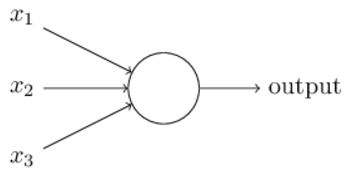
\includegraphics[scale=0.6]{Bilder/perceptron}
	\caption{Percetron mit den Eingaben $x_1, x_2, x_3$ und der Ausgabe $output$.} 
	\label{fig:perceptron} 
\end{figure}
\noindent
Für die Berechnung der Ausgabe werden sogenannte \textit{Weights} $w_n$ mit $n \in \{1, \cdots, n\}$ eingeführt, welche die Gewichtung der jeweiligen Eingabe festlegen. Der Ausgabewerte $\mathtt{output}$ wird mittels der gewichteten Summe $\sum_j w_j x_k$ und einem definierten Grenzwert $\mathtt{threshold}$ bestimmt.
\begin{equation}
	\mathtt{output} := \left\{
	\begin{array}{ll}
 		0 & \displaystyle \mbox{falls}\quad \sum\limits_j w_j x_j \leq \mathtt{threshold} \\[0.5cm]
 		1 & \displaystyle \mbox{falls}\quad \sum\limits_j w_j x_j > \mathtt{threshold}
	\end{array}\right.
\end{equation}
Werden die \textit{Weights} und der \textit{Threshold} variiert, entstehen unterschiedliche Modelle zur Entscheidungsfindung. Hierbei ist zu beachten, dass eine Minimierung des \textit{Thresholds} den binären Ausgabewert 1 mit einer höheren Wahrscheinlichkeit bedingt. \\

\noindent
Der Aufbau des Netzwerks leitet sich aus den unterschiedlichen Modellen der Entscheidungsfindung ab und wird mit Hilfe der Perceptrons abgebildet (siehe Abb. \ref{fig:perceptron_models}).
\begin{figure}[hbt]
	\centering
	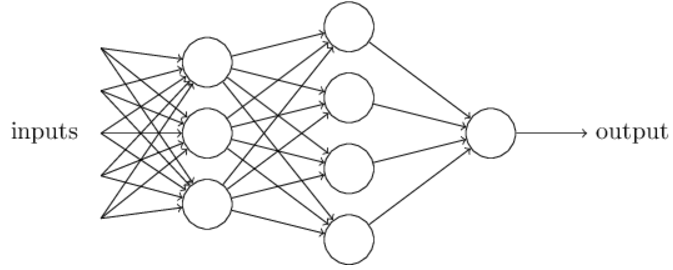
\includegraphics[scale=0.75]{Bilder/perceptron_models}
	\caption{Unterschiedliche Möglichkeiten der Entscheidungsfindung.} 
	\label{fig:perceptron_models} 
\end{figure}
Eine Entscheidungsmöglichkeit wird hierbei durch das Perceptron dargestellt. Weiterhin wird eine Spalte von Perceptrons als \textit{Layer} bezeichnet. Der erste Layer fällt Entscheidungen auf Basis der Eingabewerte, indem er diese abwägt. Jedes Perceptron des zweiten Layers hingegen, wägt für die Entscheidungsfindung die Resultate des ersten Layers ab. Ein Perceptron auf dem zweiten Layer kann somit eine Entscheidung auf einer abstrakteren und komplexeren Ebene durchführen. Auf diese Weise kann sich ein vielschichtiges Netzwerk von Perceptrons in ein anspruchsvolles Modell zur Entscheidungsfindung entwickeln. \\

\noindent
Im folgenden wird die mathematische Beschreibung von Perceptrons vereinfacht, indem Änderungen an der Notation für $\sum_j w_j x_j > \mathtt{threshold}$ vorgenommen werden. Für die Beschreibung der Summe $\sum_j w_j x_j$ werden die Vektoren $w$ und $x$ eingeführt, wodurch sich die Schreibweise $w \cdot x \equiv \sum_j w_j x_j$ ergibt. Des Weiteren wird der $\mathtt{threshold}$ auf die andere Seite der Ungleichung gezogen und erhält die Bezeichnung \textit{Bias}, $b \equiv \mathtt{-threshold}$. 
\begin{equation}
	\mathtt{output} := \left\{
	\begin{array}{ll}
 		0 & \displaystyle \mbox{falls}\quad w \cdot x + b \leq 0 \\[0.2cm]
 		1 & \displaystyle \mbox{falls}\quad w \cdot x + b > 0
	\end{array}\right.
\end{equation}
Somit nimmt der Bias Einfluss auf die binäre Ausgabe $\mathtt{output}$, weshalb der Bias eine Ausgabe mit einem hohen positiven oder negativen Wert mit einer höheren Wahrscheinlichkeit bedingen kann. \\

\noindent
Im vorherigen Abschnitt wurden Perceptrons als ein Methode für die Entscheidungsfindung beschrieben. Ein weiterer Anwendungsfall besteht in der Berechnung von logischen Funktion wie z.B. $\mathtt{AND}$, $\mathtt{OR}$ und $\mathtt{NAND}$. Fällt die Betrachtung auf ein Perceptron mit 2 Eingaben deren Gewichtung jeweils den Wert -2 aufweisen und einen Bias von 3, so ergibt sich folgende Abbildung (siehe Abb. \ref{fig:perceptron_example}).
\begin{figure}[hbt]
	\centering
	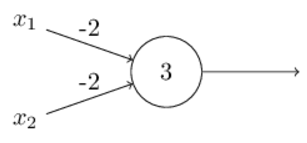
\includegraphics[scale=0.6]{Bilder/perceptron_example}
	\caption{Percetron mit zwei Eingaben -2 und einem Bias von 3.} 
	\label{fig:perceptron_example} 
\end{figure}

\noindent
Weisen die Eingaben $x_1, x_2$ den Wert 0 auf, ergibt sich für den $\mathtt{output}$ den Wert 1. Sind die Eingabewerte für $x_1, x_2$ -1 ergibt sich für den $\mathtt{output}$ den Wert -1. Der Aufbau beschreibt somit einen $\mathtt{NAND}$ Gatter.\\[0.2cm]
\hspace*{1.3cm}
$
\begin{array}[t]{lcll}
	w \cdot x + b & = & \mathtt{output} \\[0.2cm]
	(-2)*0+(-2)*0+3 & = & 1 \\[0.2cm]
	(-2)*1+(-2)*1+3 & = & -1
\end{array}
$
\\[0.2cm]
$\mathtt{NAND}$ Gatter können verwendet werden, um die unterschiedlichsten Berechnungen durchzuführen. Im Folgenden fällt die Betrachtung auf die Addition von zwei Bits $x_1$ und $x_2$. Für die Berechnung wird die bitweise Summe $x_1 \oplus x_2$ gebildet, wobei ein $\mathtt{carry bit}$ den Wert 1 annimmt, sobald $x_1$ und $x_2$ gleich 1.
\begin{figure}[hbt]
	\centering
	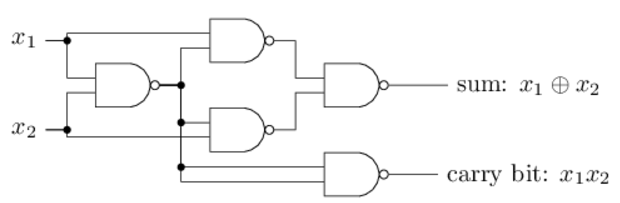
\includegraphics[scale=0.6]{Bilder/nand_gatter}
	\caption{$\mathtt{NAND}$ Gatter mit den Eingaben $x_1$ und $x_2$.} 
	\label{fig:nand_gatter} 
\end{figure}

\noindent
Um ein gleichwertiges Netzwerk abzuleiten, werden die $\mathtt{NAND}$ Gatter durch Perceptrons mit jeweils 2 Eingaben ersetzt. Hierbei weisen die Gewichtungen $w_1, w_2$ den Wert -2 und der Bias $b$ den Wert 3 auf. 
\begin{figure}[hbt]
	\centering
	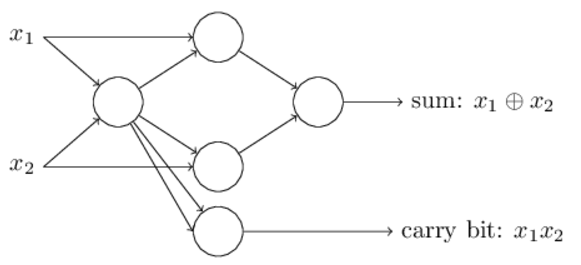
\includegraphics[scale=0.6]{Bilder/nand_gatter_perceptron}
	\caption{$\mathtt{NAND}$ Gatter Aufbau mit Perceptrons.} 
	\label{fig:nand_gatter_perceptron} 
\end{figure}

\noindent
In einem weiteren Schritt wird die Abbildung eines $\mathtt{NAND}$ Gatter mit Perceptrons vereinfacht. Dazu werden mehrere Eingänge eines Perceptrons zu einem zusammengefasst, weshalb aus den zwei Eingaben -2 der Wert -4 resultiert. Ebenfalls werden die Eingaben in einem sogenannten \textit{Input Layer} zusammengefasst, wobei durch die Notation eine Eingabe nicht mit einem Perceptron gleichzustellen ist.
\begin{figure}[hbt]
	\centering
	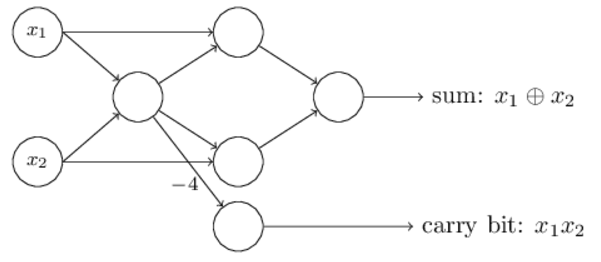
\includegraphics[scale=0.6]{Bilder/nand_gatter_perceptron_simplified}
	\caption{Vereinfachter $\mathtt{NAND}$ Gatter Aufbau mit Perceptrons.} 
	\label{fig:nand_gatter_perceptron_simplified} 
\end{figure}

\noindent
Dieser Anwendungsfall zeigt, dass mit Perceptrons unterschiedliche Berechnungen durchgeführt werden können. Implementierte Lernalgorithmen können Gewichtungen sowie den Bias automatisch durch entsprechende Stimuli im Netzwerk anpassen und ermöglichen die Nutzung von künstliche Neuronen, die sich von herkömmlichen Logik Gattern unterscheiden. Neuronale Netze können somit über einen definierten Zeitraum lernen, wie bestimmte Probleme zu lösen sind. 

\section{Sigmoid Neurons}
Für die Entwicklung lernender Algorithmen in einem Netzwerk mit Perceptrons, fällt unsere Betrachtung auf das Beispiel der Erkennung von handgeschriebenen Zahlen. Die Eingabe für das Netzwerk könnten die Raw Pixeldaten der eingescannten Bilder darstellen, welche die handgeschriebenen Zahlen abbilden. Das Ziel an dieser Stelle ist, dass das Netzwerk anhand der Veränderungen von \textit{Weights} und \textit{Biases} lernt eine korrekte Klassifizierung der Zahlen vorzunehmen. \\
Das Modifizieren der \textit{Weights} und \textit{Biases} kann das Verhalten des Netzwerkes und deren Entscheidungsfindung zu Problemen beeinflussen. Angenommen die Erkennung und Klassifizierung einer Zahl wurde durch das Netzwerk falsch vorgenommen, so können durch kleine Veränderungen an den \textit{Weights} und \textit{Biases} eine Korrektur durchgeführt werden. Dieses stetige Modifizieren der Werte über einen definierten Zeitraum ermöglicht ein lernendes Netzwerk (siehe Abb. \ref{fig:sigmoid_learning}). 
\begin{figure}[hbt]
	\centering
	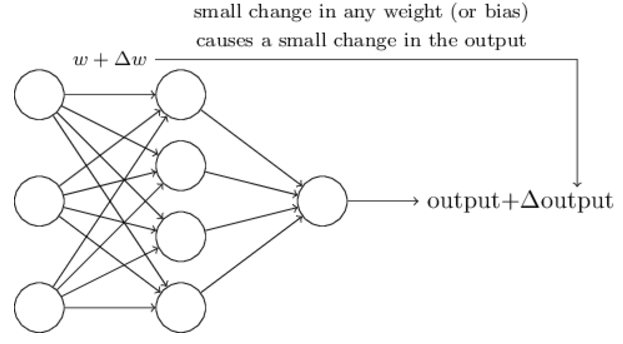
\includegraphics[scale=0.6]{Bilder/sigmoid_learning}
	\caption{Modifizieren von Weights und Biases schaffen lernendes Netzwerk.} 
	\label{fig:sigmoid_learning} 
\end{figure}

\noindent
Dieses wünschenswerte Verhalten eines lernenden Netzwerks kann durch Perceptrons nicht gewährleistet werden, da eine Veränderung der Weights und Biases den Ausgabewerte $\mathtt{output}$ eines Neurons umkehren kann. Dadurch kann das komplette Verhalten zur Klassifizierung von Zahlen beeinflusst werden, wobei zuvor falsch erkannte Zahlen nun richtig klassifiziert werden und umgekehrt. Mit Hilfe der Einführung des Sigmoid Neurons soll dieser Fehler behoben werden. Eine Änderung der Weights und Biases bei diesem künstlichen Neuron soll nur marginale Änderungen an dem Ausgabewert $\mathtt{output}$ vornehmen. Diese Erweiterung des Neurons begünstigt ein Netzwerk selbständig die Klassifizierung von Zahlen zu optimieren. \\

\noindent
Der Aufbau des Sigmoid Neurons ähnelt dem Perceptron, wobei das Neuron eine Anzahl von Eingabewerten $x_n$ mit $n \in {1, .. n}$ entgegennimmt und ausgehend von diesen Informationen den $\mathtt{output}$ ermittelt. Der wesentliche Unterschied zwischen diesen zwei Typen von Neuronen liegt in dem Wertebereich des $\mathtt{output}$.